The four layers of Smart Cart shall interface as follows. The Power supply shall interface with the cart at both the kill and the manual mode switches. It shall interface with the Imaging and navigation layer at the camera interface and with the crab drive layer at the drive system interface. The crab dive shall interface with the cat at the wheels and the imaging and navigation layer at the camera interface. 
\newpage
\begin{figure}[h!]
	\centering
 	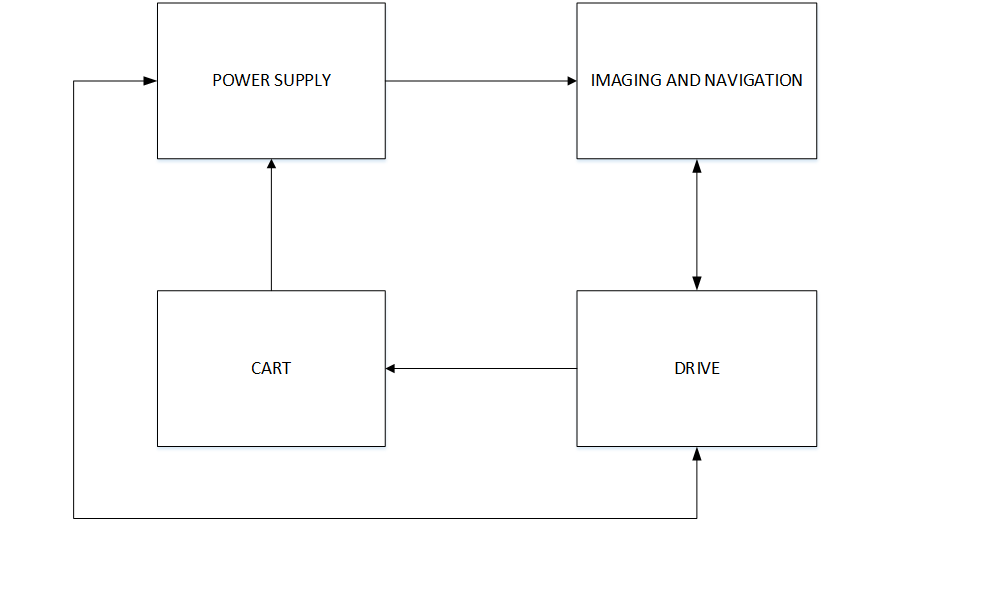
\includegraphics[width=0.90\textwidth]{images/SMART_CART}
 \caption{System architecture}
\end{figure}
\subsection{POWER SUPPLY LAYER}
Shall include a 12 volt deep cycle battery, a voltage regulator, a voltage converter and a recharge switch. The main function of this layer shall be to provide power to the rest of the layers and also to provide power for charging and powering on tools
\subsection{CART LAYER}
Shall include hardware components such as the cart, wheels, a kill switch and a manual mode switch. This shall be the cart to be driven by the crab drive, powered by the power supply and guided by the imaging and navigation layers
\subsection{CRAB DRIVE LAYER}
Shall include the motor control system, the drive system interface and the chain system. This component shall be responsible for driving the cart from one point to another
\subsection{IMAGING LAYER}
Shall include mainly the camera and the camera interface and shall be responsible for guiding the cart towards it's master and away from obstacles. 

